\documentclass[t]{beamer}

% Load general definitions
% Preamble file - general definitions, package loading, etc.

%=================================
% Load packages
\usepackage{amssymb,amsmath}
\usepackage{graphicx}
\usepackage{url}
\usepackage{tikz}
\usetikzlibrary{mindmap,trees,arrows}
\usepackage{fancyvrb}
\usepackage[english]{babel}
\usepackage[latin1]{inputenc}
\usepackage{subfigure}
\usepackage{times}
\usepackage[T1]{fontenc}
\usepackage{cancel}
\usepackage{color}
\usepackage{listings}

%=================================
% Set mode
\mode<presentation>
{
	\usetheme{Madrid}
	\usecolortheme{whale}
	\useoutertheme{infolines}
	\setbeamercovered{invisible}
}

% Get rid of nav bar
\beamertemplatenavigationsymbolsempty

% Insert frame number at bottom of the page.
\usefoottemplate{\hfil\tiny{\color{black!90}\insertframenumber}} 

%=================================
% Define new commands

\newcommand\Real{{\mathbb{R}}}
%\newcommand{\vi}{\vspace{0.6\baselineskip}}
%\newcommand{\goodgap}{\hspace{\subfigtopskip}\hspace{\subfigbottomskip}}


% Equation environments
\newcommand{\beq}{\begin{equation}}
\newcommand{\eq}{\end{equation}}
\newcommand{\beqs}{\begin{equation*}}
\newcommand{\eqs}{\end{equation*}}
\newcommand{\beqn}{\begin{eqnarray}}
\newcommand{\eqn}{\end{eqnarray}}

% Bold variables
\newcommand{\mbf}[1]{\ensuremath{\mathbf{#1}}}

% Itemization
\newcommand{\bitem}{\begin{itemize}}
\newcommand{\eitem}{\end{itemize}}
\newcommand{\spitem}{\vskip 1em\item}
\newcommand{\bitems}{\begin{itemize}\item}
\newcommand{\benums}{\begin{enumerate}\item}
\newcommand{\eenum}{\end{enumerate}}

% color blocks
\newenvironment{colorblock}[2]{%
\setbeamercolor{block title}{#2}
\begin{block}{#1}}{\end{block}}

% Vertical spacing
\newcommand{\vone}{\vskip 1em}
\newcommand{\vhalf}{\vskip .5em}

% Frame environments
\newenvironment{ftst}[3][t]{%
\begin{frame}{environment=ftst,#1}
\frametitle{#2}
\framesubtitle{#3}}{\end{frame}}

\newenvironment{ftstf}[2]{
\begin{frame}[fragile,environment=ftstf]
\frametitle{#1}
\framesubtitle{#2}}{\end{frame}}

% colors
\definecolor{MyGray}{rgb}{0.5,0.5,0.5}
\definecolor{MyDBGray}{rgb}{0.1,0.1,0.4}
\definecolor{darkgreen}{rgb}{0,0.4,0}
\definecolor{black}{rgb}{0,0,0}
\def\defn#1{{\color{red} #1}}

% Footnote
\renewcommand{\thefootnote}{\alph{footnote}}

% Relaxed footnotes
\newcommand{\lfr}[1]{\let\thefootnote\relax\footnote{\tiny #1}}

% Verbatim environment - using FANCYVRB package
\DefineVerbatimEnvironment%
{rcode}{Verbatim}
{fontsize=\scriptsize}

% Verbatim environment - using LISTINGS package
%\lstnewenvironment{rcode} {\lstset{	language = R,
%									basicstyle = \scriptsize\ttfamily,
%									showspaces = false,
%									showstringspaces = false,
%									showtabs = false,
%									keywordstyle = \color{black}\bfseries,
%									commentstyle = \color{darkgreen},
%									numbers = none,
%									otherkeywords={	<-,
%													ggplot,
%													geom_boxplot,
%													facet_grid,
%													shapiro.test,
%													fligner.test,
%													glht,
%													with},
%									deletekeywords={data,
%													model,
%													residuals,
%													c,
%													axis,
%													default,
%													labels,
%													qq.text}}}%
%{}


% Specific definitions
\title[]{Design and Analysis of Experiments}
\subtitle[]{11 - Blocking}
\author[]{Felipe Campelo\\{\footnotesize http://www.cpdee.ufmg.br/\textasciitilde fcampelo}}
\institute{Graduate Program in Electrical Engineering}
\date{\scriptsize Belo Horizonte\\May 2015}

\begin{document}

% cover page
\setbeamertemplate{footline}{}
\begin{frame}
\begin{flushright}

\includegraphics[width=.25\textwidth]{../figs/principal_completa3_ufmg}
\end{flushright}
  \titlepage
  \begin{tikzpicture}[remember picture,overlay]
  \node[anchor=south east,xshift=-5pt,yshift=122pt] at (current page.south east) {\tiny Version 2.11};
  \node[anchor=south west,yshift=0pt] at (current page.south west) {
\includegraphics[width=.15\textwidth]{../figs/by-nc-sa.png}};
  \end{tikzpicture}  
\end{frame}

%=====

% quotation page
  \begin{frame}[b]
		\frametitle{}
\begin{columns}[T]
\column{0.75\textwidth}
\flushright{\small ``\textit{Science doesn't always go forwards. It's a bit\\
like doing a Rubik's cube. You sometimes have\\
to make more of a mess with a Rubik's cube\\
before you can get it to go right.}''
\vskip 3.2em
Jocelyn Bell Burnell\\
1943 -\\
Irish astrophysicist\\}
\column{0.25\textwidth}
\begin{tikzpicture}[remember picture,overlay]
\node[anchor=south east,yshift=23pt,xshift=0pt] at (current page.south east)
{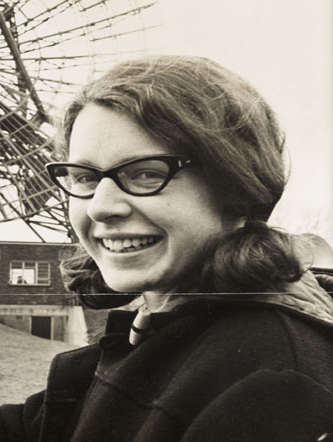
\includegraphics[width=\textwidth]{../figs/BellBurnell.png}};
\end{tikzpicture}
\end{columns}
\vhalf
\lfr{Image: \url{http://www.topbritishinnovations.org/PastInnovations/DiscoveryofPulsars.aspx}}
\end{frame}

%=====
% Main slides

\begin{ftst}
{Randomized Complete Block Design}
{Nuisance factors}
In the completely randomized design (CRD) introduced in the last chapter, the observations are assigned - as the name implies -in a completely random manner.
\vone
Implicitly, we assume that the experimental conditions are homogeneous, i.e., that no other important effects are present besides those of the experimental factor.
\vone
In some situations, however, the experiment may present other factors that are not of immediate interest, but that can influence the response variable. This was already discussed when we introduced the concept of \textit{pairing} in Chapter 7.
\end{ftst}

%=====

\begin{ftst}
{Randomized Complete Block Design}
{Nuisance factors}
The generalization of the \textit{paired design} for an arbitrary number of factor levels is called \textit{blocking}, which is an elegant way configure the data collection in order to enable the modeling and exclusion of the effects of nuisance factors.
\vone
In fact, it can be argued that the systematic use of blocking is beneficial even in the absence of known nuisance factors, as it 
\begin{columns}
	\column[T]{0.005\textwidth}
	\column[T]{0.53\textwidth}
		\vspace{-0.12em}
		helps boosting statistical power by excluding the between-replicates variability from the residual term.
	\column[T]{0.43\textwidth}
		\vspace{-0.5em}
		\begin{block}{} %{bg=green!90,fg=black}
			``\textit{\scriptsize Block what you can,\\
			\vspace{-0.5em}randomize what you cannot.}''\\
			\vhalf
			{\tiny George E.P. Box (1919--2013)\\
			\vspace{-1em}British Statistician}
			\begin{tikzpicture}[remember picture,overlay]
				\node[anchor=south east,yshift=77pt,xshift=-19pt] at (current page.south east) {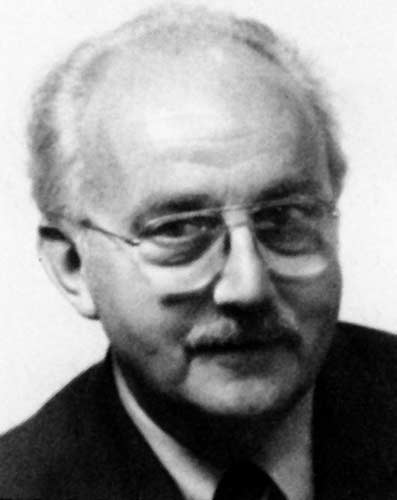
\includegraphics[width=.23\textwidth]{../figs/box.png}};
			\end{tikzpicture}
		\end{block}
	\column[T]{0.035\textwidth}
\end{columns}
\lfr{Image: \url{https://www.engr.wisc.edu/eday/eday1990.html}}
\end{ftst}

%=====

\begin{ftst}
{Randomized Complete Block Design}
{Blocking \textit{versus} Randomizing}
The idea behind randomization is trying to prevent unknown factors to bias our observations;
\vone
Blocking comes into play whenever we know from the beginning that certain factors can influence our response variable, but for some reason we are not interested in their effects\footnote[1]{\tiny If we're interested in their effects, they are no longer nuisance factors, but additional experimental factors. We'll deal with factorial designs in the next chapter.}, for instance:
\vhalf
\bitems the effect of different batches of raw material when comparing the performance of chemical reactions;
\spitem the effect of different benchmark problems when comparing the performance of computer algorithms.
\eitem
\end{ftst}

%=====

\begin{ftst}
{Example: algorithm comparison}
{Problem definition}
A Ph.D. student decides to compare a standard optimization algorithm with six modified versions for the solution of a certain family of Vehicle Routing Problems (VRPs). His intention is to verify whether any of the modified versions is systematically better than the standard one.
\vone
The algorithms are applied for the solution of 180 problem instances, divided in 36 groups of five homogeneous instances. The algorithms are run 30 times on each instance, and the cost value found after each run is recorded.
\begin{tikzpicture}[remember picture,overlay]
\node[anchor=south east,yshift=-10pt,xshift=5pt] at (current page.south east)
{
\includegraphics[width=.27\textwidth]{../figs/phdStudent.png}};
\end{tikzpicture}
\lfr{Image: PhD Comics by Jorge Cham:}
\lfr{\url{http://www.phdcomics.com/comics/archive.php?comicid=1139}}
\end{ftst}

%=====

\begin{ftst}
{Example: algorithm comparison}
{Nuisance factor}
Besides the effect of the experimental factor (\textit{Algorithm}), we have a possible nuisance effect due to the variability between experimental units (instance groups).
\vone
If we employ a CRD, the residual term would contain all the between-instances variability, which would almost certainly mask any between-algorithms effect of interest.
\vone
Since we can control the allocation of algorithm runs within each instance, one possibility is to do it in a systematic way so that we can model the instance effects (in addition to the factor effect).
\end{ftst}

%=====

\begin{ftst}
{Example: algorithm comparison}
{Randomized complete block design}
Within each \textit{block}, the order of execution should in principle be randomized, so as to prevent other unknown factors from affecting our analysis\footnote[2]{\tiny For this kind of computer experiment the within-block randomization is unnecessary. It is very important, however, when dealing with systems that are less controllable.}. 
\vone
This experimental setup is known as a \textit{randomized complete block design} (RCBD) with one blocking factor.
\end{ftst}

%=====

\begin{ftst}
{Randomized complete block design}
{Assumptions}
The RCBD assumes:

\bitems \textit{one replicate per block}\footnote[3]{\tiny For multiple within-block replicates the appropriate design is known as \textit{Generalized randomized block design} (GRBD), which is analyzed using a factorial model.};
\spitem independent blocks;
\spitem independent within-block randomization. 
\eitem

The RCBD assumes that each block is independent from all others - failure to account for dependency structures can result in pseudoreplication, i.e., the use of the incorrect number of degrees-of-freedom in the test statistics.
\end{ftst}

%=====

\begin{ftst}
{Example: algorithm comparison}
{RCBD}
To comply with these requirements, we consider as our response variable the average performance of an algorithm on a particular \textit{instance group}.
\vone
The performance of each algorithm will be averaged within each individual instance (mean of 30 runs), and then within each group (mean of 5 instances), so that each algorithm has 36 independent observations.
\end{ftst}

%=====

\begin{ftst}
{Analysis of the RCBD}
{Statistical model}
In the general case, we have $a$ levels of the experimental factor, and $b$ levels for the blocking factor. The statistical model is given as:

\beqs
y_{ij} = \mu + \tau_i + \beta_j + \epsilon_{ij}\begin{cases}
i=1,\ldots,a\\
j=1,\ldots,b
\end{cases},\ \mbox{assuming }\epsilon_{ij}\sim\mathcal{N}\left(0,\sigma^2\right)
\eqs
\vone

Similarly to the CRD we have, by construction: 
\begin{align*}
\sum\limits_{i=1}^a\tau_i = 0\ \ \ \ \ \ \ \ \ \ \ \ \ \sum\limits_{j=1}^{b}\beta_j = 0
\end{align*}
\end{ftst}

%=====

\begin{ftst}
{Analysis of the RCBD}
{Statistical model}
In the RCBD, we are interested only on the effect of the experimental factor. Consequently, the test hypotheses refer only to its coefficients:

\beqs
\begin{cases}
H_0: \tau_i = 0,\ \ \forall i=1,\cdots,a \\
H_1: \exists\ \tau_i\neq 0
\end{cases}
\eqs

The partition of the total sample variability is given by:
\begin{align*}
SS_T 	&= \sum\limits_{i=1}^{a}\sum\limits_{j=1}^{b}{\left(y_{ij} - \bar{y}_{\cdot\cdot}\right)^2}\\
		&= \underbrace{b\sum\limits_{i=1}^{a}{\left(\bar{y}_{i\cdot} - \bar{y}_{\cdot\cdot}\right)^2}}_{SS_{\mbox{\tiny levels}}} + \underbrace{a\sum\limits_{j=1}^{b}{\left(\bar{y}_{\cdot j} - \bar{y}_{\cdot\cdot}\right)^2}}_{SS_{\mbox{\tiny blocks}}} +\underbrace{\sum\limits_{i=1}^{a}\sum\limits_{j=1}^{b}{\left(y_{ij} - \bar{y}_{i\cdot} - \bar{y}_{\cdot j} + \bar{y}_{\cdot\cdot}\right)^2}}_{\tiny SS_E}
\end{align*}
\end{ftst}

%=====

\begin{ftst}
{Analysis of the RCBD}
{Statistical model}
The mean squares are given by:

\begin{align*}
MS_{\mbox{\tiny levels}} &= \frac{SS_{\mbox{\tiny levels}}}{a-1} &MS_{\mbox{\tiny blocks}} &= \frac{SS_{\mbox{\tiny blocks}}}{b-1}	& MS_{E} &= \frac{SS_{E}}{(a-1)(b-1)}\\
\end{align*}

\noindent and their expected values are:
\begin{align*}
E\left[MS_{\mbox{\tiny levels}}\right] &= \sigma^2 + \frac{b\sum\limits_{i=1}^{a}\tau_i^2}{a-1}	&	&E\left[MS_{\mbox{\tiny blocks}}\right] &= \sigma^2 + \frac{a\sum\limits_{j=1}^{b}\beta_j^2}{b-1}\\&&&&\\ & & E\left[MS_{E}\right] &= \sigma^2 & \ 
\end{align*}
\end{ftst}

%=====

\begin{ftst}
{Analysis of the RCBD}
{Statistical model}
\beqs
E\left[MS_{\mbox{\tiny levels}}\right] = \sigma^2 + \frac{b\sum\limits_{i=1}^{a}\tau_i^2}{a-1}	\ \ \ \ \ \ \ \ \ \ \ \ \ \ \ E\left[MS_{E}\right] = \sigma^2
\eqs

Under the null hypotheses we have that the test statistic
\beqs 
F_0 = \frac{MS_{\mbox{\tiny levels}}}{MS_E} 
\eqs

\noindent is a distributed according to an $F$ distribution with $(a-1)$ numerator degrees-of-freedom and $(a-1)(b-1)$ denominator DoFs.
\vone
The critical region for the test is therefore given by
\vone
\centering $f_0 > F_{\alpha; (a-1),\left(a-1\right)\left(b-1\right)}$
\end{ftst}

%=====

\begin{ftst}
{Analysis of the RCBD}
{Multiple blocking factors}
If there is more than one factor that need to be blocked out of the analysis, it is possible to simply add new terms to the statistical model. The sum of squares for this new term is similar to the ones already shown for the single block case;
\vone
However, since we are not really interested in the block effects - all we want is to get them out of our residual term - we can use the \textit{KISS} principle\footnote[4]{\tiny``\textit{\textbf{K}eep \textbf{I}t \textbf{S}imple, \textbf{S}tupid!}'', as introduced by American engineer C.L. ``Kelly'' Johnson in the 1970's. If one wants to be more polite, there is a quote attributed to Einstein that reads ``\textit{Make everything as simple as possible, but not simpler}'', but the acronym MEASAPBNS is just not as catchy.}, merge the two (or more) blocking factors into a single one and proceed with the analysis as if only one blocking factor actually existed.
\end{ftst}

%=====

\begin{ftst}
{Analysis of the RCBD}
{Blocking efficiency}
After an experiment is performed and the ANOVA model is fit to the data, it is possible to calculate the \textit{relative blocking efficiency} ($E$), which quantifies how much larger a CRD would have to be in order to attain the same power as the corresponding RCBD.
\vone
The relative efficiency can be calculated from the mean squares returned in the ANOVA table of the RCBD as:

\beqs
E = \frac{(b-1)MS_{\mbox{\tiny Blocks}} + b(a-1)MS_{\mbox{\tiny E}}}{(ab-1)MS_{\mbox{\tiny E}}}
\eqs
\vhalf
A value of 1.3, for instance, would indicate that the CRD would have required $30\%$ more observations to achieve the same power.
\end{ftst}

%=====

\begin{ftst}
{Analysis of the RCBD}
{Sample size calculations}
The determination of the required sample size for an RCBD follows the same procedures as the CRD: the number of replicates calculated using the CRD formulas represent the number of blocks required (since we have one replicate per block).
\vone
The within-group variability term necessary for calculating the required sample size corresponds to the estimated residual variance, i.e., the unexplained variability after accounting for the experimental and blocking factors, which can be somewhat challenging to estimate without a information on previous studies (or a pilot experiment).
\end{ftst}

%=====

\begin{ftst}
{Analysis of the RCBD}
{Multiple comparisons}
For the post-hoc multiple comparison procedures, we also follow the same general guidelines used for the CRD, with some minor differences.
\vone
Paired t-tests are used for the pairwise comparisons, with $df_E = (a-1)(b-1)$ as the number of degrees of freedom used for the reference distributions;
\vone
As with the CRD, it may be convenient to use the post-hoc pairwise comparison procedures as the basis for sample size calculations, particularly in cases where the cost of observations is relatively low.
\end{ftst}


\begin{ftst}
{Bibliography}
{\ }
\scriptsize
\textbf{Required reading}

\benums  
\eenum

\textbf{Recommended reading}

\benums 
\eenum
\end{ftst}

%=====

\begin{ftstf}{About this material}{Conditions of use and referencing}
\centering\footnotesize This work is licensed under the Creative Commons CC BY-NC-SA 4.0 license\\(Attribution Non-Commercial Share Alike International License version 4.0).\\
\vhalf
\url{http://creativecommons.org/licenses/by-nc-sa/4.0/}\\
\vone
\footnotesize Please reference this work as:\\
\footnotesize \flushleft Felipe Campelo (2015), \textit{Lecture Notes on Design and Analysis of Experiments}.\\Online: {\scriptsize\url{https://github.com/fcampelo/Design-and-Analysis-of-Experiments}}\\
Version 2.11, Chapter 11; Creative Commons BY-NC-SA 4.0.\\

\begin{Verbatim}[fontsize=\tiny]
    @Misc{Campelo2015-01,
      title={Lecture Notes on Design and Analysis of Experiments},
      author={Felipe Campelo},
      howPublished={\url{https://github.com/fcampelo/Design-and-Analysis-of-Experiments}},
      year={2015},
      note={Version 2.11, Chapter 11; Creative Commons BY-NC-SA 4.0.},
    }
\end{Verbatim}

\begin{tikzpicture} [remember picture,overlay]
\node[anchor=south,yshift=0pt] at (current page.south){ \includegraphics[width=.2\textwidth]{../figs/CCSomerights.png}};
\end{tikzpicture}
\end{ftstf}


\end{document}